
%%%%%%%%%%%%%%%%%%
%                %
% Introduction   %
%                %
\chapter{Introduction}
\label{cp:intro}

%\begin{highlight}
%    \begin{st}
%        General structure with just some dummy text.
%    \end{st} 
%\end{highlight}

\lettrine{M}{obile robots} are a class of robots with the ability to move through the environment~\citep{corke2017robotics}. Most of these robots are power-demanding devices constrained by battery limitations. Whilst such limitations are a common challenge in many areas, they are critical in mobile robots' design and development. They impact the level of autonomy~\citep{seewald2020mechanical}, which in turn is expected to increase in the foreseeable future~\citep{fisher2013verifying}.

To move, mobile robots combine different components which sense and interact with the surrounding environment~\citep{mei2006deployment}. The analysis and interpretation of data originating from these components require energy-demanding heterogeneous computing hardware. Planning an energy-aware path with a power-saving scheduling policy on such hardware is an underrepresented topic in the literature. In fact, many past approaches focus almost exclusively on one of these topics. For instance, some generate an energy-optimized path, despite the energy needed for the computations almost equaling the actuation in some instances of low-energy mobile robots~\citep{sudhakar2020balancing}. Due to the recent advancements in the computational capabilities of mobile hardware, such as the introduction of powerful portable GPUs~\citep{rizvi2017general}, the use of computations is expected to increase~\citep{abramov2012real,satria2016real,jaramillo2019visual}. Other approaches provide a power-saving scheduling policy. Yet, actuating a mobile robot requires considerable power over mere calculations~\citep{mei2004energy,mei2005case}.

In this work, we focus on energy optimal planning for the path and scheduling for the computational tasks. We plan these two aspects simultaneously, exploring their tradeoffs. We demonstrate the approach both in simulation and empirically focusing on aerial mobile robots. These systems share with the broader class of mobile robots very stringent battery limitations. Recharging the battery during normal operation is, however, rarely an option for aerial robots. It would require to land to replace or recharge the battery~\citep{zamanakos2020energy}. They are hence a perfect instance of energy constrained and they well apply to an energy optimization planning approach.

We first build an energy model to predict the future energy consumption of some autonomous operations. We then estimate the coefficients of the model using robust estimation techniques. We later derive an optimal configuration of the path and computations using modern optimal control. We use the optimal configuration to derive guidance and scheduling actions for an aerial mobile robot. The guidance allows us to move physically the aerial robot; the scheduling defines the granularity of the tasks being executed in flight.

\begin{figure}[t]
  \centering
  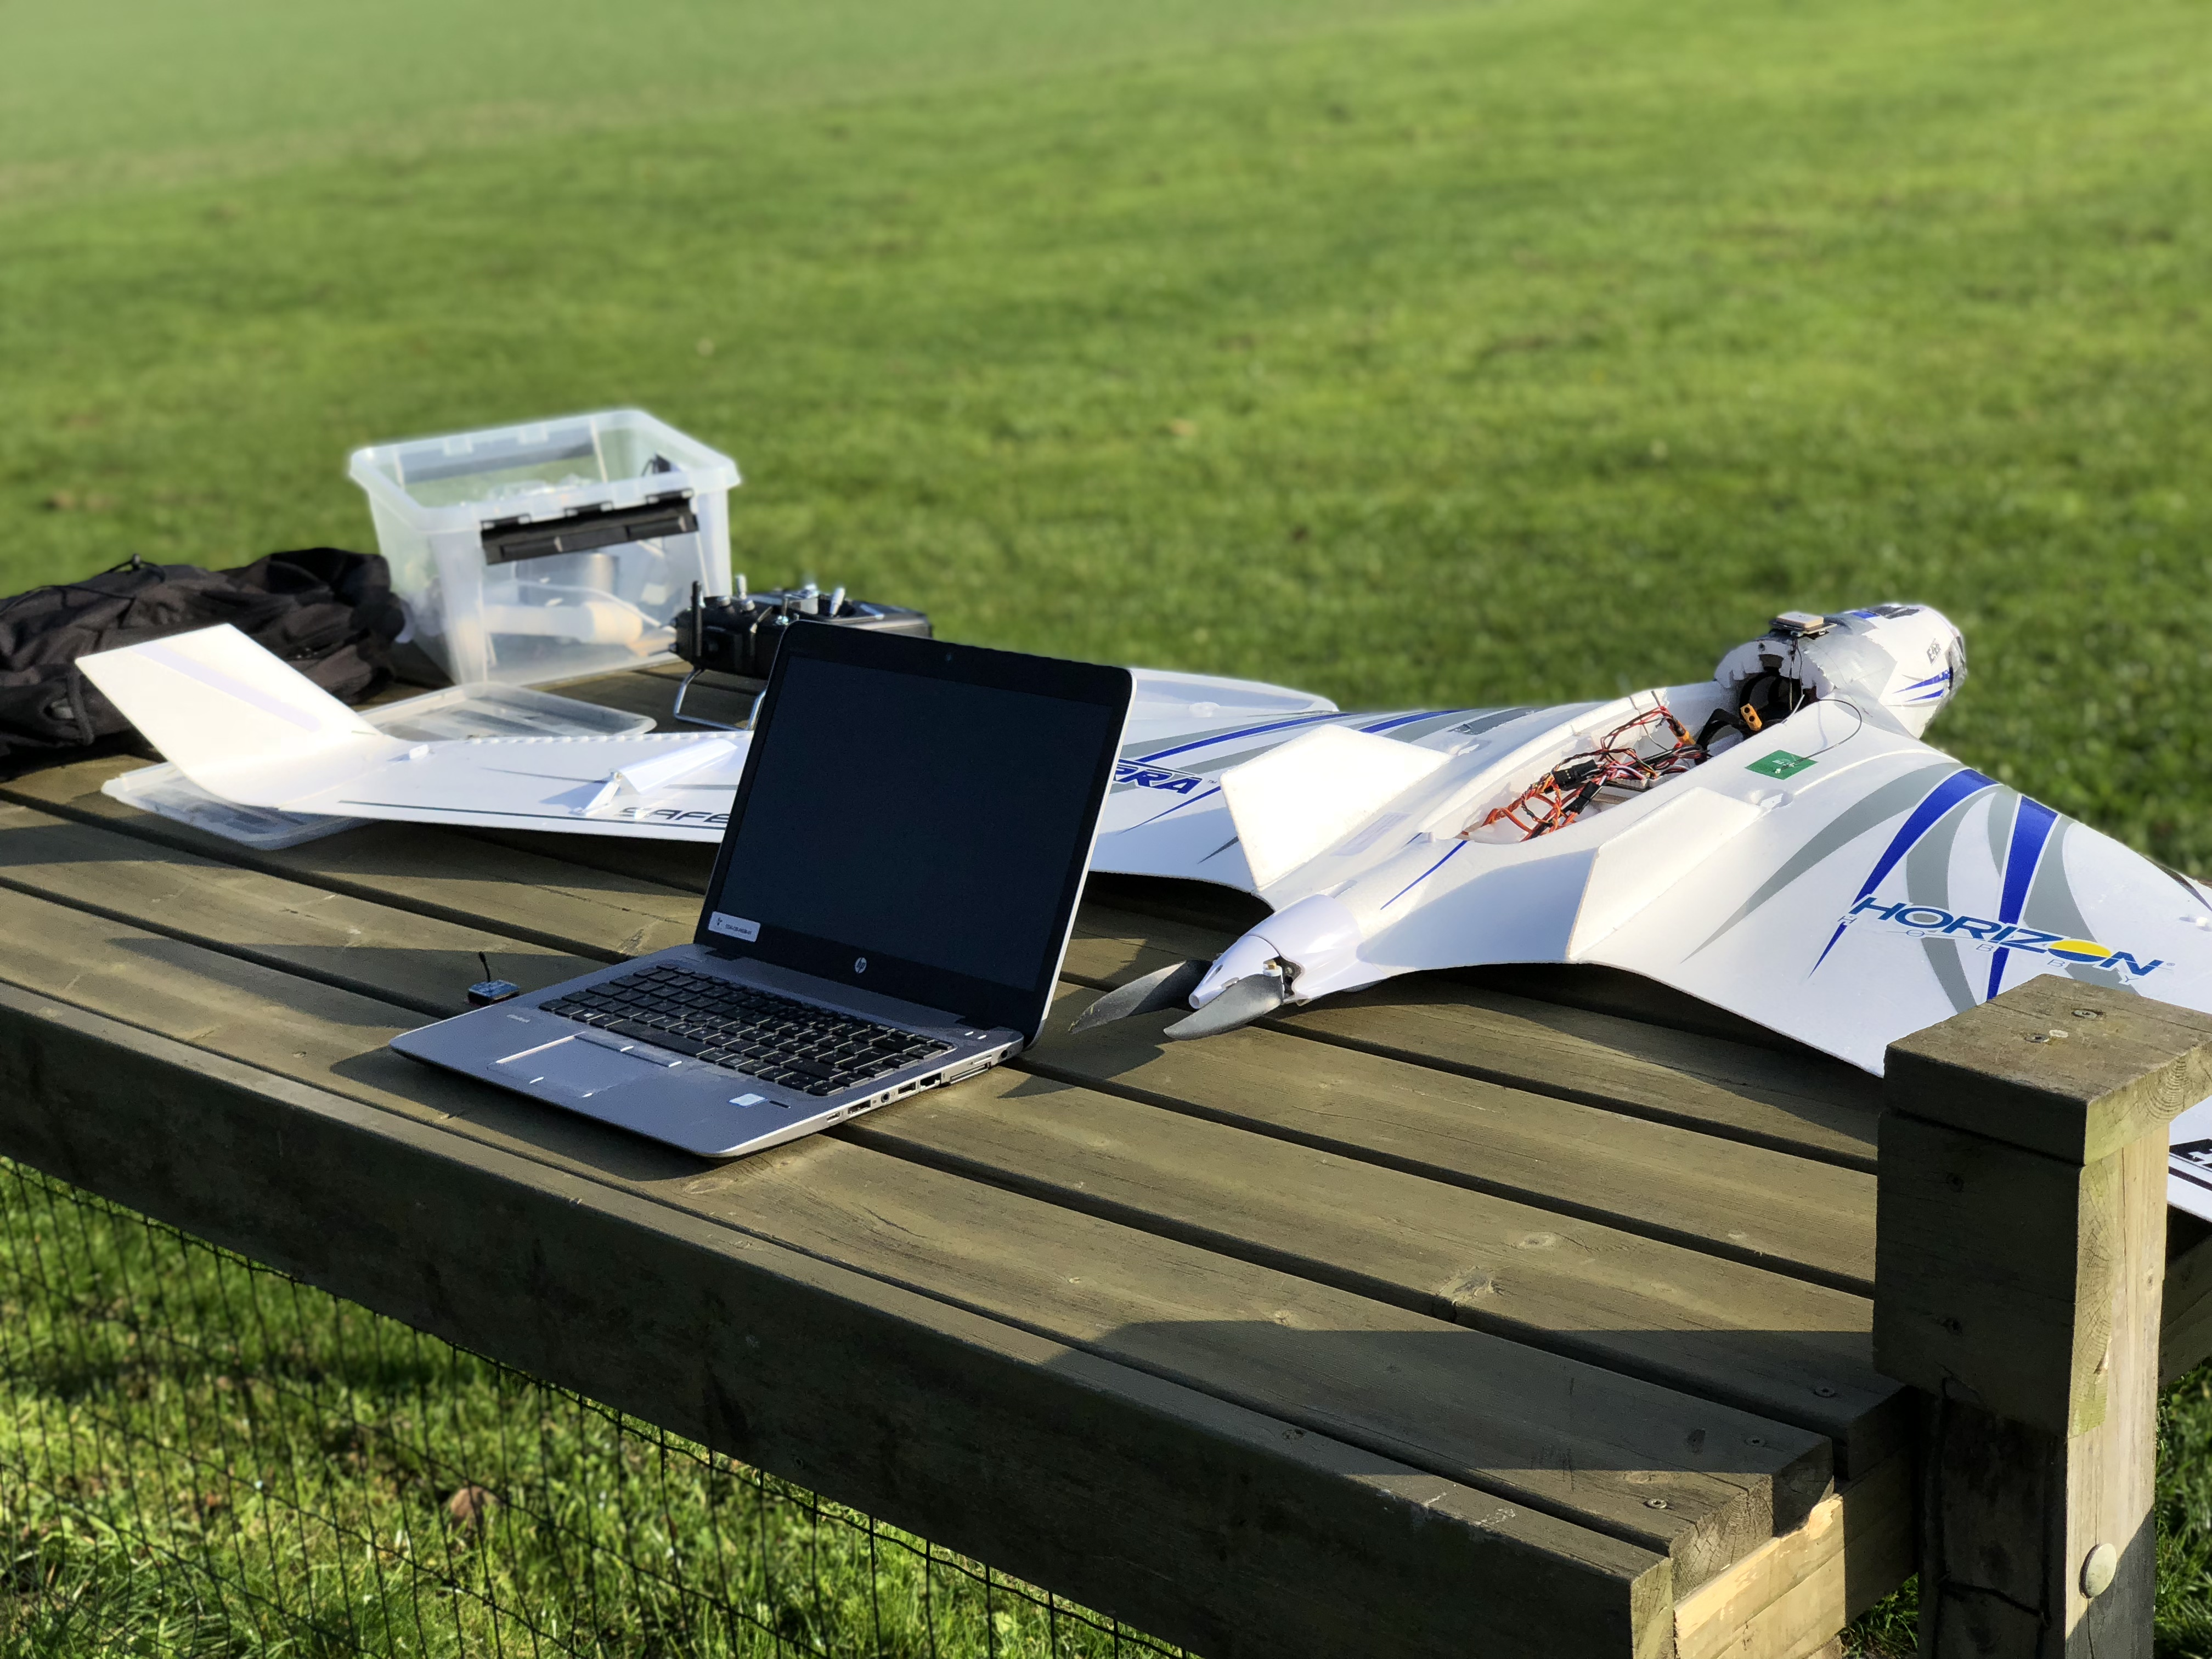
\includegraphics[width=.7\textwidth]{pictures/photo}
  \caption[Opterra fixed-wing UAV]{Opterra fixed-wing UAV employed as an aerial robotics platform for precision agriculture. Photo credit: Amit Ferencz Appel.}   
  \label{fig:opterra}
\end{figure}

The aerial robotics platform we investigate most in this work is the Opterra fixed-wing \Gls{acr:uav}~\citep{opterra} adapted for precision agriculture. Precision agriculture is often put into practice~\citep{hajjaj2014review} with ground mobile robots used for harvesting~\citep{qingchun2012study,dong2011development, de2011design, aljanobi2010setup, li2008analysis, edan2000robotic}, and \Gls{acr:uav}s for preventing damage and ensuring better crop quality~\citep{puri2017agriculture, daponte2019review}. The aerial robot, is shown in \fref{fig:opterra}{Figure}.

\section{From UAVs to Modern Aerial Robots}

Modern aerial robots are a valuable tool in robotic research and aerospace. Historically, they can be found with different names in the literature. These include unmanned aerial vehicles\findex{unmanned aerial vehicles} (\Gls{acr:uav}s)\footnote{The term unmanned is sometimes replaced by uninhabited if the vehicle is operated remotely by human operator}%citation to anderson
, unmanned aerial systems\findex{unmanned aerial systems} (\Gls{acr:uas}s), flying robots, or drones. Usually, we refer to drones, \Gls{acr:uav}s, and \Gls{acr:uas}s when these systems are semi-autonomous, or operated from the ground (\Gls{acr:uas} often denote the entire infrastructure of unmanned flight in the aerospace jargon). Aerial or flying robots, on the other hand, have advanced levels of autonomy~\citep{siciliano2016springer}. Nevertheless, all these systems have basic autonomous features such as position and altitude holding and leveling. The position holding is implemented using global navigation satellite system~\findex{global navigation satellite system} (\Gls{acr:gnss}), altitude holding using a barometer~\findex{barometer}, and leveling using inertial measurement unit~\findex{inertial measurement unit} (\Gls{acr:imu}).

\begin{figure}[t]
  \centering
  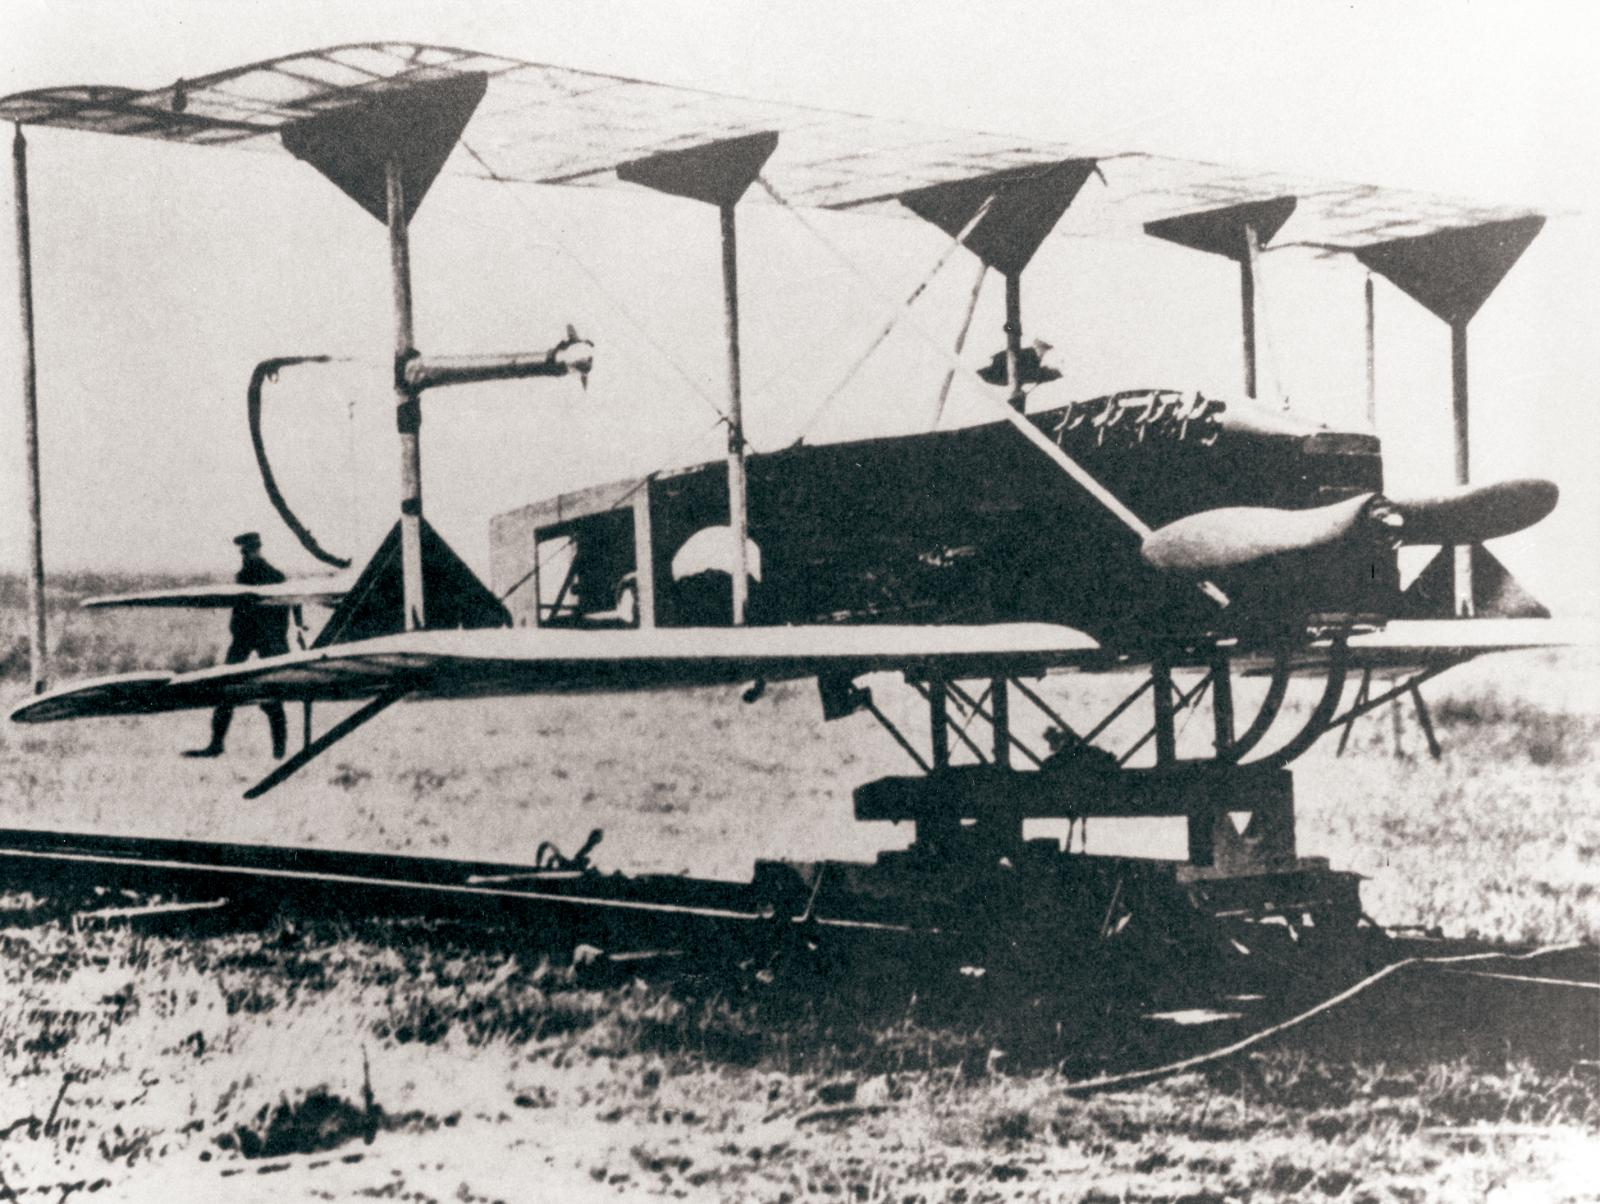
\includegraphics[width=.7\textwidth]{pictures/HA-NH-JA-19_1}
  \caption[The Hewitt-Sperry Automatic Airplane]{The Hewitt-Sperry Automatic Airplane also denomined ``flying bong'' was developed in the first world war and represents the first instance of a UAV. Photo credit: United States Naval Institute.}   
  \label{fig:opterra}
\end{figure}

Aerial robotics has more than a century of developments~\citep{siciliano2016springer}. The origin of the field of aerial robotics, which deals with design and development of aerial robots, dates back to the first guided missiles~\citep{siciliano2016springer}, although unmanned flying machines has more than a century of developments. One of the first such unmanned flying machine is the Hewitt-Sperry Automatic Airplane from the 1917~\citep{valavanis2015handbook}; a milestone reached relatively soon if we consider that the first heavier-than-air flight in history was demonstrated 14 years earlier with the Wright Flyer I by Wilbur and Orville Wright (commonly referred to as the Wright brothers). The Hewitt-Sperry Automatic Airplane used a gyroscope mechanically connected to the control surfaces thus successfully integrating a control feedback loop~\citep{siciliano2016springer}.

In  the early days, aerial robots were labeled remotely piloted vehicles~\findex{remotely piloted vehicles} (\Gls{acr:rpv}s)~\citep{anderson2005introduction}. Some instances of early aerial robots were designed for military purposes. In the 1950s, United States used a remotely controlled vehicle Ryan Firebee~\findex{Ryan Firebee} for reconnaissance in Vietnam, and Israel used first a \Gls{acr:rpv} in a combat situation~\citep{anderson2005introduction}. Some other instances of such vehicles include the V-1 flying bomb from 1944 (deployed by German armed forces), and the Lockheed D-21 from 1962.

Global positioning system (GPS) at the end of 1970 opened the possibility for using the \Gls{acr:uav}s in autonomous surveillance, and later integrate the with cameras~\citep{siciliano2016springer}, paving for the introduction of modern \Gls{acr:uav}s.

Aerial robots are used increasingly in applications such as remote sensing, surveillance, meteorology, search and rescue, precision agriculture, transportation, and payload delivery. Although the former four categories fall into the area of reconnaissance, surveillance, and target acquisition\findex{reconnaissance, surveillance, and target acquisition} (\Gls{acr:rsta}), agriculture, transportation, and payload delivery are often realized using to a greater or lesser extent some advanced levels of computational intelligence~\citep{siciliano2016springer}. Modern aerial robots are designed to handle unexplored terrain with little interaction opposed to past \Gls{acr:uav}s that were mostly operated by a human operator~\citep{siciliano2016springer}. Instances of these systems are in fact expected to autonomously adapt and possibly interact in a broad variety of environmental conditions.


%A quote from~\cite{anderson2005introduction}: ``the Wright brothers worked so hard to put humans in the air in flying machines, a hundred years later some [...] are working hard to take them out of flying machines''

\subsection{Types of aerial robots}

{\color{red}A description of the different classes of aerial robots (rotorcrafts, fixed-wings, vtols...)}

\section{Motivation}

Many scenarios involving unmanned aerial vehicles (UAVs), such as precision agriculture, search and rescue, and surveillance, require high autonomy but have limited energy budgets. A typical example of these scenarios is a UAV following a path and performing some on-board computational tasks. For instance, the UAV might detect ground patterns and notify other ground-based actors with little human interaction. We refer to such computational tasks that can be dynamically replanned and adapted as \emph{computations}. We are interested in the energy optimization of the path and computations under uncertainty (atmospheric interferences) and refer to it as energy-aware dynamic planning. Such planning would find optimal tradeoffs between the path, computations, and energy requirements. Current generic planning solutions for outdoor UAVs do not plan the path and computations dynamically, nor are they energy-aware. They are often semi-autonomous: the path and computations are static and usually defined using planning software~\citep{daponte2019review} (for instance~\citep{papa} and~\citep{px4}). Such a state of practice has prompted us to propose an \emph{energy-aware dynamic planning algorithm} for UAVs. The algorithm combines and generalizes some of the past body of knowledge on mobile robot planning problems and addresses the increasing \emph{computational demands} and their relation to energy consumption, path, and autonomy for the UAV planning problem.

\section{Objective}


\section{Outline of the Approach}

Unlike most of the past planning algorithms literature, our algorithm plans the path and computations simultaneously. To model the path we use multiple mathematical functions. For instance, the path might contain multiple circles and lines. To model the computations we use \powprof{}, a profiling tool presented in previous work~\citep{seewald2019coarse}. To guide the UAV we use a vector field~\citep{de2017guidance} that converges to the path. The use of vector fields for guidance is widely discussed in the literature~\citep{lindemann2005smoothly,gonccalves2010vector,panagou2014motion,zhou2014vector,kapitanyuk2017guiding,de2017guidance}. 


To achieve the energy-aware dynamic planning, we further introduce and formally prove a periodic energy model that accounts for the uncertainty. We use Fourier analysis to derive the model, and state estimation to address the uncertainty. Periodicity is often present due to repetitive patterns in the plan~\citep{seewald2020mechanical}. Indeed, UAV scenarios often iterate over a set of tasks and paths (e.g., monitoring or search and rescue). Given that the plan is periodic, we expect the energy consumption to approximately evolve periodically. Some collected energy data from a UAV flying a survey scenario along its power spectrum motivates our choice.

% add these plots

In the spirit of reducing costs and resources, we showcase the algorithm using dynamic planning for a precision agriculture fixed-wing UAV. Precision agriculture is often put into practice~\citep{hajjaj2014review} with ground mobile robots used for harvesting~\citep{qingchun2012study,dong2011development, de2011design, aljanobi2010setup, li2008analysis, edan2000robotic}, and UAVs for preventing damage and ensuring better crop quality~\citep{puri2017agriculture, daponte2019review}. The plan is structured as follows. Path-wise, the UAV flies in circles and lines covering a polygon. Computation-wise, it detects hazards using a neural network and notifies grounded mobile robots employed for, e.g., harvesting. The algorithm alters the plan; it controls the processing rate and the radius of the circles (affecting the distance between the lines). 

We observe that not only the path but also the computations significantly impact the energy, with a potential extension of up to 13 minutes over an hour by switching from the highest to the lowest level of computations in presence of a standard battery.

\section{Applications}

\section{Problem Formulation}
\label{cp:intro:pb}

Let us adopt the following mathematical notation. Given an integer $a$, $[a]$ is the set $\{0,1,\dots,a\}$, $[a]^+$ the set $[a]/\{0\}$. Bold lower-case letters indicates vectors. $c_{i,j}$ the $j$-th parameter of the $i$-th parameters set $c_i$. $\underline{c}_{i,j},\overline{c}_{i,j}$ are the lower and upper bounds of the parameter $c_{i,j}$.

\begin{figure}[h]
  \center
  \begin{tikzpicture}[shorten >=.5pt,node distance=12.5ex,on grid,auto]
    \node[state,initial] (q_i) {$\Gamma_1$}; 
    \node        [right=of q_i] (q_dots0) {$\cdots$};
    \node[state] (q_0) [right=of q_dots0] {$\Gamma_i$};
    \node        (q_dots1) [right=of q_0] {$\cdots$};
    \node[state,accepting] (q_f) [right=of q_dots1] {$\Gamma_f$};
    \path[->]
    (q_i) edge node {$\mathbf{p}_{\Gamma_{1}}$} (q_dots0)
    (q_dots0) edge node{$\mathbf{p}_{\Gamma_{i-1}}$} (q_0)
    (q_0) edge node {$\mathbf{p}_{\Gamma_i}$} (q_dots1)
    (q_dots1) edge node {$\mathbf{p}_{\Gamma_{l}}$} (q_f)    
    (q_i) edge [loop above] node {$\mathbf{p}_{k_1}$} (q_i)
    (q_0) edge [loop above] node {$\mathbf{p}_{k_2}$} (q_0)
    (q_f) edge [loop above] node {$\mathbf{p}_{k_3}$} (q_f)
    ; %end path 
    \draw [decorate,decoration={brace,amplitude=10pt,mirror,raise=10pt},yshift=0pt]
    (q_i.south west) -- (q_f.south west) node [black,midway,yshift=-9ex]{$\Gamma$};
  \end{tikzpicture}
  \caption{The plan defined as a FSM}
  \label{fig:state-machine}
\end{figure}

Let us assume that the path at stage $i$ can be altered with $\rho$ path parameters
\begin{equation}
    c_i^\rho:=\{c_{i,1},c_{i,2},\dots,c_{i,\rho}\},
\end{equation}
and the computations with $\sigma$ computation parameters 
\begin{equation}
    c_i^\sigma:=\{c_{i,\rho+1},c_{i,\rho+2},\dots,c_{i,\rho+\sigma}\}.
\end{equation}

We then express the path as a continuous twice differentiable function $\varphi_i:\mathbb{R}^2\times\mathbb{R}^\rho\rightarrow\mathbb{R}$ of a point and the path parameters. The function returns a metric of the distance between the point and the nominal trajectory. We express the computations as the value of the computation parameters. We discuss the concrete meaning of the value of path parameters in \fref{cp:model}{Chapter}.

\begin{highlight}  
  \begin{defn}[Stage, plan, triggering, and final point]\label{def:mission}
    The $i$-th \emph{stage} $\Gamma_i$ at time instant $k$ of a plan $\Gamma$ is defined
    \begin{equation*}\begin{split}
      \Gamma_i:=\{\varphi_i(\mathbf{p}_k,c_i^\rho),c_i^\sigma\mid
      \,&\exists\,\,\mathbf{p}_k,\,\varphi_i(\mathbf{p}_k,c_i^\rho)\in\mathcal{C}_i,\,\\
        &\,\forall j\in[\sigma]^+,\,c_{i,\rho+j}\in\mathcal{S}_{i,j}\,\},
    \end{split}\end{equation*}
    where $\mathcal{C}_i:=[\underline{c}_i,\overline{c}_i]\subseteq\mathbb{R}$ is the path constraint set, and $\mathcal{S}_{i,j}:=[\underline{c}_{i,\rho+j},\overline{c}_{i,\rho+j}]\subseteq\mathbb{Z}_{\geq 0}$ the $j$-th computation constraint set. $\mathbf{p}_k$ is a point of a UAV flying at an altitude $h\in\mathbb{R}_{>0}$ w.r.t. some inertial navigation frame $\mathcal{O}_W$.
  
    The \emph{plan} is a finite state machine (FSM) $\Gamma$ where the state-transition function $s:\bigcup_i{\Gamma_i}\times\mathbb{R}^2\rightarrow\bigcup_i{\Gamma_i}$ maps a stage and a point to the next stage
    \begin{equation*}s(\Gamma_i,\mathbf{p}_k):=\begin{cases}
      \Gamma_{i+1} & \text{if }\mathbf{p}_k=\mathbf{p}_{\Gamma_i}\\
      \Gamma_i & \text{otherwise}
    \end{cases}.\end{equation*}
    The point $\mathbf{p}_{\Gamma_{i}}$ that allows the transition between $\Gamma_i$ and $\Gamma_{i+1}$ is called \emph{triggering point}. The last triggering point $\mathbf{p}_{\Gamma_{l}}$ relative to the last stage $\Gamma_l$ is called \emph{final point}.
  \end{defn}
\end{highlight}

\begin{figure}[t]
    \centering
    
\definecolor{c989898}{RGB}{152,152,152}
\definecolor{cDEDEDE}{RGB}{222,222,222}
\definecolor{cFFFFFF}{RGB}{255,255,255}
\definecolor{c2B2B2B}{RGB}{43,43,43}
\definecolor{c9B9B9B}{RGB}{155,155,155}


\def \globalscale {1.000000}
\begin{tikzpicture}[y=0.80pt, x=0.80pt, yscale=-1.1*\globalscale, xscale=1.1*\globalscale, inner sep=0pt, outer sep=0pt]
\path[draw=c989898,line join=round,line width=0.512pt] (37.9773,138.5660) -- (35.3357,138.5630);



  \path[fill=cDEDEDE,line join=round,even odd rule,line width=0.160pt] (59.2379,138.5360) -- (37.3300,138.5360) .. controls (37.3300,104.2680) and (65.1100,76.4881) .. (99.3784,76.4881) -- (99.3784,98.1778) .. controls (77.1987,98.3164) and (59.2589,116.3290) .. (59.2379,138.5360) -- cycle;



  \path[fill=cDEDEDE,line join=round,even odd rule,line width=0.160pt] (36.8146,208.2220) -- (59.2401,208.2220) -- (59.2407,138.0860) -- (36.8151,138.0860) -- (36.8146,208.2220) -- cycle;



  \path[fill=cDEDEDE,line join=round,even odd rule,line width=0.160pt] (75.5064,138.3220) -- (53.5984,138.3220) .. controls (53.5984,104.0540) and (81.3785,76.2741) .. (115.6470,76.2741) -- (115.6470,97.9639) .. controls (93.4671,98.1025) and (75.5273,116.1150) .. (75.5064,138.3220) -- cycle;



  \path[fill=cDEDEDE,line join=round,even odd rule,line width=0.160pt] (115.5600,97.9479) -- (115.5600,76.0399) .. controls (149.8280,76.0399) and (177.7080,103.8200) .. (177.7080,138.0880) -- (156.0190,138.0880) .. controls (155.8800,115.9090) and (137.7680,97.9688) .. (115.5600,97.9479) -- cycle;



  \path[fill=cDEDEDE,line join=round,even odd rule,line width=0.160pt] (53.0716,208.2330) -- (75.4972,208.2330) -- (75.4974,138.0950) -- (53.0718,138.0950) -- (53.0716,208.2330) -- cycle;



  \path[fill=cDEDEDE,line join=round,even odd rule,line width=0.160pt] (155.9570,208.2190) -- (178.3830,208.2190) -- (178.3990,137.9630) -- (155.9730,137.9630) -- (155.9570,208.2190) -- cycle;



  \path[draw=c989898,line join=round,line width=0.512pt] (99.5543,138.9930) ellipse (1.7511cm and 1.7511cm);



  \path[cm={{1.0,0.0,0.0,1.0,(190.0,175.0)}}] (0.0000,0.0000) node[above right] () {$\mathbf{p}_{k_4}$};



    \path[fill=cFFFFFF,line join=round,line width=0.160pt,rounded corners=0.0000cm] (65.5184,186.6300) rectangle (81.7257,202.8374);



    \path[cm={{1.0,0.0,0.0,1.0,(66.0,199.0)}}] (0.0000,0.0000) node[above right] () {$\varphi_1$};



  \path[draw=c2B2B2B,line join=round,line width=0.512pt] (115.6970,138.4880) ellipse (1.7511cm and 1.7511cm);



  \path[draw=c2B2B2B,line join=round,line width=0.512pt] (53.2806,50.4116) -- (53.2808,208.0220);



  \path[draw=c2B2B2B,line join=round,line width=0.512pt] (177.8300,50.4301) -- (177.8300,208.0410);



  \path[draw=c2B2B2B,line join=round,line width=0.512pt] (118.1030,140.8340) -- (113.8230,136.5520);



  \path[draw=c2B2B2B,line join=round,line width=0.512pt] (113.8260,140.8310) -- (118.1070,136.5500);



  \path[fill=black,line join=round,line width=0.256pt] (52.5078,197.6220) -- (52.5078,192.2880) -- (53.7878,192.2880) -- (53.7878,197.6220) -- (52.5078,197.6220) -- cycle(52.5078,186.9550) -- (52.5077,181.6220) -- (53.7877,181.6220) -- (53.7877,186.9550) -- (52.5078,186.9550) -- cycle(52.5077,176.2890) -- (52.5077,170.9550) -- (53.7877,170.9550) -- (53.7877,176.2890) -- (52.5077,176.2890) -- cycle(52.5077,165.6220) -- (52.5077,160.2890) -- (53.7877,160.2890) -- (53.7877,165.6220) -- (52.5077,165.6220) -- cycle(52.5076,154.9550) -- (52.5076,149.6220) -- (53.7876,149.6220) -- (53.7876,154.9550) -- (52.5076,154.9550) -- cycle(52.5076,144.2890) -- (52.5076,138.9550) -- (53.7876,138.9550) -- (53.7876,144.2890) -- (52.5076,144.2890) -- cycle(53.0267,133.5810) -- (53.1252,132.8330) -- (53.8254,128.9130) -- (53.9747,128.2740) -- (55.2289,128.5300) -- (55.0796,129.1680) -- (54.3905,133.0260) -- (54.2992,133.7200) -- (53.0267,133.5810) -- cycle(55.2719,123.0650) -- (56.4670,119.0750) -- (56.8957,117.9440) -- (58.1090,118.3510) -- (57.6804,119.4830) -- (56.5094,123.3920) -- (55.2719,123.0650) -- cycle(58.8505,112.9310) -- (61.1435,108.1160) -- (62.3221,108.6150) -- (60.0291,113.4300) -- (58.8505,112.9310) -- cycle(63.8781,103.4730) -- (64.7913,101.9480) -- (66.9793,99.0624) -- (68.0419,99.7761) -- (65.8539,102.6620) -- (65.0079,104.0740) -- (63.8781,103.4730) -- cycle(70.4287,94.9101) -- (74.1486,91.0881) -- (75.1213,91.9201) -- (71.4014,95.7421) -- (70.4287,94.9101) -- cycle(78.4053,87.7408) -- (80.3745,86.2019) -- (82.9136,84.7517) -- (83.6288,85.8132) -- (81.0897,87.2634) -- (79.2622,88.6916) -- (78.4053,87.7408) -- cycle(87.6306,82.0689) -- (92.6007,80.1345) -- (93.1529,81.2893) -- (88.1827,83.2237) -- (87.6306,82.0689) -- cycle(97.7391,78.4275) -- (102.9360,77.2307) -- (103.3130,78.4540) -- (98.1160,79.6508) -- (97.7391,78.4275) -- cycle(108.2830,76.3988) -- (113.5950,75.9193) -- (113.7960,77.1835) -- (108.4840,77.6630) -- (108.2830,76.3988) -- cycle(119.0310,75.9276) -- (124.3360,76.4738) -- (124.2840,77.7527) -- (118.9790,77.2066) -- (119.0310,75.9276) -- cycle(129.6590,77.4030) -- (134.8450,78.6494) -- (134.6300,79.9113) -- (129.4440,78.6648) -- (129.6590,77.4030) -- cycle(139.9380,80.4796) -- (144.0440,82.1042) -- (144.9200,82.6049) -- (144.3640,83.7578) -- (143.4890,83.2571) -- (139.5520,81.7000) -- (139.9380,80.4796) -- cycle(149.5490,85.2532) -- (150.9890,86.0768) -- (153.9650,88.3831) -- (153.2520,89.4460) -- (150.2750,87.1396) -- (148.9930,86.4062) -- (149.5490,85.2532) -- cycle(158.1060,91.8657) -- (161.8580,95.6554) -- (161.0080,96.6118) -- (157.2550,92.8221) -- (158.1060,91.8657) -- cycle(165.1950,99.9168) -- (166.1480,101.1420) -- (168.1780,104.4180) -- (167.1250,105.1460) -- (165.0960,101.8700) -- (164.2320,100.7590) -- (165.1950,99.9168) -- cycle(170.7940,109.1320) -- (172.2860,112.1330) -- (173.0420,114.0250) -- (171.8730,114.5450) -- (171.1170,112.6530) -- (169.6740,109.7510) -- (170.7940,109.1320) -- cycle(174.9250,119.0630) -- (175.9740,122.3380) -- (176.4510,124.2150) -- (175.2200,124.5650) -- (174.7430,122.6880) -- (173.7200,119.4930) -- (174.9250,119.0630) -- cycle(177.6310,129.4510) -- (177.8280,130.4450) -- (178.2610,133.3030) -- (178.4240,134.7830) -- (177.1550,134.9460) -- (176.9910,133.4660) -- (176.5670,130.6630) -- (176.3820,129.7310) -- (177.6310,129.4510) -- cycle(178.5140,140.1950) -- (178.5100,145.5280) -- (177.2300,145.5270) -- (177.2340,140.1940) -- (178.5140,140.1950) -- cycle(178.5060,150.8610) -- (178.5020,156.1950) -- (177.2220,156.1940) -- (177.2260,150.8600) -- (178.5060,150.8610) -- cycle(178.4970,161.5280) -- (178.4930,166.8610) -- (177.2130,166.8600) -- (177.2170,161.5270) -- (178.4970,161.5280) -- cycle(178.4890,172.1950) -- (178.4850,177.5280) -- (177.2050,177.5270) -- (177.2090,172.1940) -- (178.4890,172.1950) -- cycle(178.4810,182.8610) -- (178.4800,184.3970) -- (177.2000,184.3960) -- (177.2010,182.8600) -- (178.4810,182.8610) -- cycle(52.5078,208.2880) -- (52.5078,202.9550) -- (53.7878,202.9550) -- (53.7878,208.2880) -- (52.5078,208.2880) -- cycle;



    \path[fill=cFFFFFF,line join=round,line width=0.160pt,rounded corners=0.0000cm] (170.4340,62.4618) rectangle (186.6414,78.6691);



    \path[cm={{1.0,0.0,0.0,1.0,(170.0,75.0)}}] (0.0000,0.0000) node[above right] () {$\varphi_4$};



  \path[fill=cFFFFFF,line join=round,line width=0.160pt,rounded corners=0.0000cm] (151.1930,87.1333) rectangle (167.4004,103.3407);



  \path[cm={{1.0,0.0,0.0,1.0,(154.0,98.0)}}] (0.0000,0.0000) node[above right] () {$\varphi_5$};



  \path[cm={{1.0,0.0,0.0,1.0,(16.0,120.0)}}] (0.0000,0.0000) node[above right] () {$\mathbf{p}_{k_3}$};



  \path[draw=c989898,line join=round,line width=0.512pt] (101.6410,140.7130) -- (97.3588,136.4310);



  \path[draw=c989898,line join=round,line width=0.512pt] (97.3620,140.7090) -- (101.6430,136.4300);



  \path[draw=c989898,line join=round,line width=0.512pt] (37.4683,50.2362) -- (37.4674,207.8470);



  \path[draw=black,line join=round,line width=1.024pt] (37.3655,139.1460) .. controls (37.3655,108.3180) and (59.8482,82.7404) .. (89.3117,77.9160);



  \path[draw=black,line join=round,line width=1.024pt] (37.4074,138.8430) -- (37.4612,139.4260);



  \path[draw=black,line join=round,line width=1.024pt] (104.8160,14.6465) .. controls (114.1410,17.1626) and (116.3470,26.7356) .. (116.3470,26.7355) .. controls (116.3470,26.7355) and (134.0140,69.7724) .. (87.7439,78.3357);



  \path[draw=black,fill=cFFFFFF,line join=round,line width=0.512pt] (38.0214,129.9470) -- (48.4265,113.7660) -- (41.6299,114.7590) -- (36.4969,110.7700) -- (38.0214,129.9470) -- cycle;



  \path[draw=black,line join=round,line width=1.024pt] (37.3995,208.3130) -- (37.3999,138.8280);



    \path[fill=cFFFFFF,line join=round,line width=0.160pt,rounded corners=0.0000cm] (48.2360,62.4618) rectangle (64.4433,78.6691);



    \path[cm={{1.0,0.0,0.0,1.0,(46.0,75.0)}}] (0.0000,0.0000) node[above right] () {$\varphi_6$};



  \path[draw=black,line join=round,line width=0.512pt] (38.2486,129.1090) -- (41.5789,114.8440);



  \path[draw=black,fill=cFFFFFF,line join=round,line width=0.512pt] (75.8501,81.3976) -- (95.0620,82.3957) -- (90.0278,77.8124) -- (91.7396,70.5527) -- (75.8501,81.3976) -- cycle;



  \path[draw=black,line join=round,line width=0.512pt] (76.2742,81.2804) -- (89.9006,77.8114);



  \path[draw=black,line join=round,line width=1.024pt] (177.8490,208.2210) -- (177.8490,158.6520);



  \path[draw=black,fill=c9B9B9B,line join=round,line width=0.512pt] (177.8340,156.5720) -- (171.4330,174.7140) -- (177.8190,172.1830) -- (183.7320,174.8830) -- (177.8340,156.5720) -- cycle;



  \path[draw=black,line join=round,line width=0.512pt] (177.8060,157.4410) -- (177.8490,172.0900);



  \path[draw=black,fill=cFFFFFF,line join=round,line width=0.512pt] (122.5820,36.7240) -- (118.0690,18.0488) -- (113.9380,22.8537) -- (107.6780,24.6001) -- (122.5820,36.7240) -- cycle;



  \path[draw=black,line join=round,line width=0.512pt] (11.2790,8.9418) -- (11.2790,38.5413);



  \path[draw=black,line join=round,line width=0.512pt] (40.6757,38.3017) -- (11.0761,38.3017);



  \path[cm={{1.0,0.0,0.0,1.0,(1.0,52.0)}}] (0.0000,0.0000) node[above right] () {$\mathcal{O}_W$};



  \path[draw=black,line join=round,line width=0.512pt] (12.2122,38.1596) -- (114.5840,24.7774);



    \path[fill=cFFFFFF,line join=round,line width=0.160pt,rounded corners=0.0000cm] (49.3746,20.2690) rectangle (73.7139,36.4553);



    \path[cm={{1.0,0.0,0.0,1.0,(53.0,35.0)}}] (0.0000,0.0000) node[above right] () {$\mathbf{p}_{k_1}$};



  \path[draw=black,line join=round,line width=0.512pt] (113.9240,22.8546) -- (122.4610,36.6020);



  \path[fill=black,line join=round,line width=0.160pt] (38.7120,35.2069) -- (38.7201,41.3379) -- (44.3321,38.2655) -- (38.7120,35.2069) -- cycle;



  \path[fill=black,line join=round,line width=0.160pt] (8.2258,10.6325) -- (14.3568,10.6281) -- (11.2877,5.0143) -- (8.2258,10.6325) -- cycle;



  \path[fill=black,line join=round,line width=0.160pt] (109.5870,22.7566) -- (110.5860,28.8056) -- (115.6270,24.8662) -- (109.5870,22.7566) -- cycle;



    \path[fill=cFFFFFF,line join=round,line width=0.160pt,rounded corners=0.0000cm] (29.9808,62.4618) rectangle (46.1881,78.6691);



    \path[cm={{1.0,0.0,0.0,1.0,(27.0,75.0)}}] (0.0000,0.0000) node[above right] () {$\varphi_2$};



\path[draw=c2B2B2B,line join=round,line width=0.512pt] (179.6380,138.6350) -- (177.4990,138.6330);



\path[draw=c2B2B2B,line join=round,line width=0.512pt] (53.7370,138.6060) -- (51.0981,138.6060);



  \path[fill=cFFFFFF,line join=round,line width=0.160pt] (185.5880,202.9890) -- (173.1380,202.9890) -- (173.1040,215.0630) -- (185.5830,215.0320) -- (185.5880,202.9890) -- cycle;



  \path[cm={{1.0,0.0,0.0,1.0,(176.0,213.0)}}] (0.0000,0.0000) node[above right] () {$\overline{c}_4$};



  \path[fill=cFFFFFF,line join=round,line width=0.160pt] (160.5750,202.9910) -- (148.1260,202.9910) -- (148.0920,215.0660) -- (160.5710,215.0350) -- (160.5750,202.9910) -- cycle;



  \path[cm={{1.0,0.0,0.0,1.0,(151.0,213.0)}}] (0.0000,0.0000) node[above right] () {$\underline{c}_4$};




\path[cm={{1.0,0.0,0.0,1.0,(14.0,143.0)}}] (0.0000,0.0000) node[above right] () {$\mathbf{p}_{\Gamma_1}$};



\path[fill=cFFFFFF,line join=round,line width=0.160pt,rounded corners=0.0000cm] (62.9567,132.2440) rectangle (79.1640,148.4513);



\path[cm={{1.0,0.0,0.0,1.0,(66.0,144.0)}}] (0.0000,0.0000) node[above right] () {$\mathbf{p}_{\Gamma_5}$};



\path[cm={{1.0,0.0,0.0,1.0,(183.0,143.0)}}] (0.0000,0.0000) node[above right] () {$\mathbf{p}_{\Gamma_4}$};



\path[draw=black,line join=round,line width=0.512pt] (99.5120,138.7510) -- (99.5120,76.7023);



\path[fill=black,line join=round,line width=0.160pt] (97.1960,80.5069) -- (101.9120,80.5006) -- (99.5490,76.1842) -- (97.1960,80.5069) -- cycle;



  \path[fill=cFFFFFF,line join=round,line width=0.160pt] (108.2100,108.6570) -- (90.4810,108.6560) -- (90.4810,121.1060) -- (108.2100,121.1060) -- (108.2100,108.6570) -- cycle;



  \path[cm={{1.0,0.0,0.0,1.0,(93.0,120.0)}}] (0.0000,0.0000) node[above right] () {$c_{1,1}$};




\end{tikzpicture}


    \caption[Definition notation on a slice of the plan]{Definition notation shown on an slice of the plan.}
    \label{fig:traj1}
\end{figure}

The altitude $h$ from \fref{def:mission}{Definition} might change at different flying phases and under different atmospheric conditions

In \fref{fig:traj1}{Figure}, $\varphi_1,\dots,\varphi_6$ are paths. $\varphi_1$ and $\varphi_5$ are circles, while $\varphi_2$, $\varphi_4$, and $\varphi_6$ are lines. They are all relative to different stages $\Gamma_1,\Gamma_2,\dots$. The constraints set $\mathcal{C}_1,\mathcal{C}_2,\dots$ forms the area where the paths $\varphi_1,\varphi_2,\dots$ can be altered with the parameters $c_{i,1},\dots,c_{i,\rho}$ (gray area in the figure). This area is bounded by $\underline{c}_i,\overline{c}_i$, and can be different per each stage \fref{fig:traj1}{Figure}, the area relative to $\Gamma_4$ is bounded by $\underline{c}_4,\overline{c}_4$).

In \fref{fig:traj1}{Figure}, $\mathbf{p}_{\Gamma_1}$ allows the transition between $\Gamma_1$ and $\Gamma_2$, $\mathbf{p}_{\Gamma_4}$ between $\Gamma_4$ and $\Gamma_5$, and $\mathbf{p}_{\Gamma_5}$ between $\Gamma_5$ and $\Gamma_6$.

A slice of the plan in \fref{fig:state-machine}{Figure} shows the transition between the stages with the FSM. The triggering point $\mathbf{p}_{\Gamma_{i-1}}$ allows the transition to the stage $\Gamma_i$. The UAV remains in the stage with any generic point $\mathbf{p}_{k_2}$. It eventually enters the stage $\Gamma_{i+1}$ with the triggering point $\mathbf{p}_{\Gamma_i}$ and so on, until it reaches the final point. The stage $\Gamma_f$ is the accepting stage (it indicates that the UAV has completed the plan).

\begin{figure}[h]
  \center
  \begin{tikzpicture}[shorten >=1pt,node distance=27ex,on grid,auto] 
    \node        (q_dots0) {$\cdots$};
    \node[state] (q_0) [right=of q_dots0] {$\Gamma_i$};
    \node        (q_dots1) [right=of q_0] {$\cdots$};   
    \path[->]
    (q_dots0) edge node{$\mathbf{p}_{\Gamma_{i-1}}(c_1^\rho,\dots,c_{i-1}^\rho)$} (q_0)
    (q_0) edge node {$\mathbf{p}_{\Gamma_i}(c_1^\rho,\dots,c_{i}^\rho)$} (q_dots1)    
    (q_0) edge [loop above] node {$\mathbf{p}_{k}$} (q_0)
    ; %end path
  \end{tikzpicture}
\caption[Detail of a stage in the FSM]{Detail of the stage $\Gamma_i$ in the FSM}
\label{fig:state-machine2}
\end{figure}
    
Generally, one can express the triggering points in function of the $i$-th trajectory parameters $c_{i}^{\rho}$, or any previous trajectory parameters, propagating the information therein if necessary (see \fref{fig:state-machine2}{Figure}).
   

\subsection{Problem formulation}

In order to simplify the problem formulation, we consider some primitive paths. All the other paths are built from these paths with a shift $\mathbf{d}:=(x_d,y_d)$.

Given $n\in\mathbb{Z}_{>0}$ ($n<l,l/n\in\mathbb{Z}$) primitive paths $\varphi_1,\dots\varphi_n$, a generic starting point $\mathbf{p}$ and the current levels of the path parameters $c_1^\rho$, all the other paths $\varphi_{n+1},\dots,\varphi_l$ are built
\begin{equation}\label{eq:primitive}\begin{split}
  &\varphi_{(i-1)n+j}(\mathbf{p}+(i-1)\mathbf{d},c_1^\rho)-\\ &\,\,\,\varphi_{in+j}(\mathbf{p}+i\mathbf{d},c_1^\rho)=e_j,
\end{split}\end{equation}
$\forall i\in[l/n-1]^+,j\in[n]^+$, where $e_j\in\mathbb{R}$ is the $j$-th constant difference.

\begin{highlight}
\begin{defn}[Period]\label{def:period}
  The period $T\in\mathbb{R}_{> 0}$ is the time between $\varphi_{(i-1)n+j}$ and $\varphi_{in+j}$ in \frefeq{eq:primitive}.
\end{defn} 
\end{highlight}

The algorithm measures the time between the paths and assumes the initial period is one. The periods might be different for different $j$s due to atmospheric interferences.

One can define the plan using primitive paths or define all the stages explicitly and find $n$ searching the value which satisfies the \frefeq{eq:primitive}. If there is no such value, (e.g., when the plan is composed of only one stage), the period $T$ from \fref{def:period}{Definition} can be determined empirically from energy data.

\begin{highlight}
\begin{pb}[UAV planning problem]\label{pb}
  Consider an initial plan $\Gamma$ from \fref{def:mission}{Definition}. We are interested in the planning of the parameters $c_i,\,\forall i\in[l]^+$ and energy constraints and in the guidance of the UAV to the path resulting from such plan.
\end{pb}    
\end{highlight}

\section{Structure}

